%!TEX encoding=UTF-8 Unicode
%!TEX root=../tabarnac.tex

\section{TABARNAC}
\label{sec:design}

\TABARNAC is divided into two parts: the instrumentation tool and the
visualization.  In this section, we discuss the implementation of both parts.

\subsection{Instrumentation}
\label{sec:design-impl}

The instrumentation part of \TABARNAC is based on a custom memory tracer for the Pin Dynamic Binary Instrumentation~(DBI) tool~\cite{Luk05Pin}.
Before running the application, our tool retrieves static memory allocation
informations using the library \texttt{libelfg0}. Dynamic allocations are
intercepted with a \texttt{malloc} replacement. If the application is
compiled with debug flags (\texttt{-g}), the structure names that are malloc'ed can be extracted from the source
code. If we can not retrieve a structure name, we call it
\texttt{AnonymousStruc\#ID}, where $ID$ is a unique identifier for the
execution, starting at $0$. Finally, each time a thread is created, we compute
its stack bounds, and create a virtual structure named \texttt{Stack\#N} where
$N$ is the thread id. Only structures that are bigger than one page (usually
$4$Kib) are recorded as our
analysis granularity is the memory page. The data structure informations (name,
size and address) are not used during the instrumentation, they are only
printed in a file at the end of the analysis to be used by the visualization
tool.

During the execution, our tracer intercepts every memory access of the parallel application.
For each access, we store the type of access (read or write), the memory page that was accessed, and the thread ID.
The information is stored on a per-thread basis, as shown in
Listing~\ref{lst:mem}, making the code completely lock-free as well as minimizing the amount of false sharing.

%\begin{figure}[!h]
\begin{lstlisting}[caption=Code that is executed on each memory access.,label=lst:mem]
	void mem_access(uint64_t address, uint32_t threadid, char type)
	{
		uint64_t page = address >> page_bits;
		acc[threadid][page][type]++;
	}

\end{lstlisting}
%\caption{Code that is executed on each memory access.}
%\label{fig:code}
%\end{figure}


At the end of the tracing phase, we generate two \texttt{csv} files.
The first file contains the list of pages and the number of reads
and writes per threads. The second file contains the
list of structures with their names, sizes and start addresses.
We then call an R-markdown script which will first read the two csv files and
retrieve the page / data structure mapping, then generate the final
visualization presented in Section~\ref{sec:design-visu}. We use R-markdown
for the visualization as it allows us to interleave plots with plain text
explanation and optimization hints.

% not relevant I'd say:
% \TABARNAC have very few dependencies and can be installed easily. If all the R
% library required to generate the visualization are not present, our tool is
% able to install them automatically. By default \TABARNAC generate the memory
% trace and the visualization, but the user can also choose to only generate the
% memory trace or the visualization. This is useful for people who cannot
% install R on the machine used to generate the trace. Moreover it allows the
% user to customize the plots generate by the R script.

\subsection{Visualization}
\label{sec:design-visu}

Providing an easy to read visualization of a memory trace is a challenge. We opted for an
assisted visualization. Once the analyze phase is done, \TABARNAC will
generate an HTML page, providing a summary of the trace through several plots.
This HTML page is generated using R markdown as well.
Before each plot, we explain how to read it, what
usual issues it can help to understand and we give hints on how to fix the issues.

The visualization starts with a small introduction, reminding the main
principles while developing for NUMA machines, then it shows the analysis
machine's topology using Hwloc~\cite{Broquedis10hwloc}.

In the next part, the visualization focuses on data structures usage. Some structures might
be ignored for two reason: either no accesses have been detected during the
analysis, which happens for structures used by external libraries, or less than 0.01\% of the total accesses happens on them. This is done to make the output
more readable. However, it is possible to ask \TABARNAC not to ignore
structures in the second case.

The first series of plots aims to give information concerning the relative
importance of data structures. It shows the size of each data structure and the
number reads and writes done by each thread on each structure. The global
read/write pattern is also displayed. These plots gives a general idea of the
structures used by threads, it allows also to identify master/slave patterns.
Moreover, knowing the read/write behavior is very useful as it determines the
possible optimization. For instance, structures written only at initialization
(or very rarely) can be (relatively) easily duplicated in a way that each NUMA
node works on a local copy.
\DB{Maybe to much details here ?}

The second series of plots is the most important one, it shows for
each thread and each structure the distribution of accesses inside the
structure. It gives an easy way to understand data sharing between threads and
structures usage. The plots presented in Sections~\ref{sec:exp-mat}~and~\ref{sec:exp-is} come from this series. They can be used to identify inefficient memory usage or to determine the best NUMA mapping
policy.

Finally, \TABARNAC provides a plot that shows for each page of each structure
which thread was responsible for the first touch (this information is used in Section~\ref{sec:exp-ondes3d}, for example). This information is quite relevant as the default
policy for Linux is to map a page as close as possible to the first thread
accessing it. If the first touch distribution doest not fit the actual access
distribution, the default mapping done by \emph{Linux} might not be efficient.
To improve this issue, the developer can either distribute correctly the first touch or do some
manual data mapping to ensure better memory access locality during the execution.

\subsection{Analysis overhead}
\label{sec:expe-overhead}

\begin{figure}[htb]
    \centering
    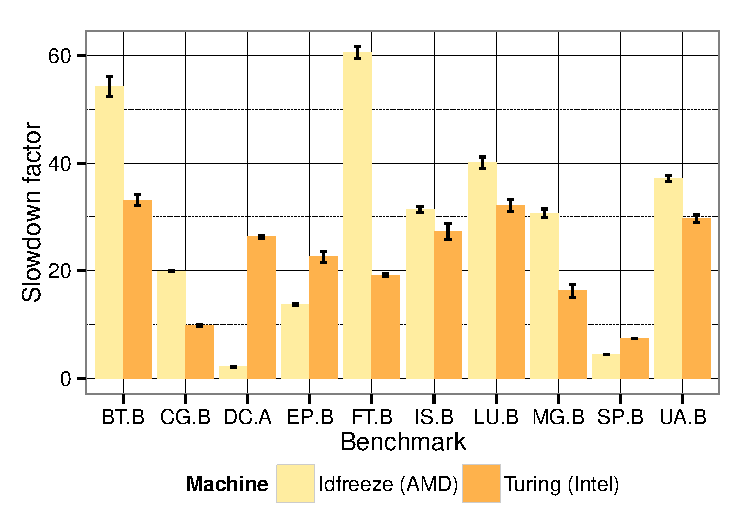
\includegraphics[width=.4\textwidth]{tool-ovh.pdf}
    \caption{Overhead of \TABARNAC~ analysis for the NAS Parallel Benchmarks.}
    \label{fig:ovh}
\end{figure}

To evaluate the instrumentation overhead, we ran all the NAS Parallel Benchmarks in
class B with 64 threads on our experimental machine (see Section~\ref{sec:metho}) and compared the original execution time with the
execution time under instrumentation. We can see in Figure~\ref{fig:ovh} that
the instrumentation is $10$ to $30$ times slower than the normal execution. Although it is
no negligible, we have to consider the fact that often we can instrument
smaller version of the applications as we focus on the general behavior.
Moreover as we do not use sampling, our instrumentation is deterministic and
there is no need to run several times the instrumentation. Finally as our
analysis is designed to be used during the development phase of the
application and not by an automated tool during the execution, even a factor $30$
is quite reasonable.
\itodo{should probably be in the results section}
